\chapter{Organisational Vision and Goals}
\label{cap:visiongoals}

%   Savas
\section{Vision}
The Banks's organisational vision is focused on business expansion, digital transformation, and international growth. To achieve this vision, the executive board established several objectives, including increasing the domestic retail banking market share from 7\% to 10\%, increasing internet banking revenue by 70\%, increasing revenue generated from customers outside the headquarters country by 50\%, and achieving a 5\% increase in corporate profit. 

The business vison is based on the integration of newly acquired banks, the expansion of strategic partnerships, and the automation and standardisation of business and IT operations. Consequently, Information Technology becomes a strategic enabler rather than a support function. To support the organisational vision, the IT department aims to operate as a Shared Service Center capable of delivering high-performance, high-quality, and cost-effective services. This transformation requires the adoption of a \textbf{Performance-Based Management} approach, where service performance is continuously measured, monitored, and improved through data-driven decision making. The strategic direction of the IT department is therefore built around three Critical Success Factors: Customer Partnership, Process Factory, and Continuous Improvement.


%   Still working on it its gonna grow

\section{Goals}

% • Focus on value 
% • Start where you are 
% • Progress iteratively with feedback 
% • Collaborate and promote visibility  
% • Think and work holistically
% • Keep it simple and practical 
% • Optimize and automate 


The acquisition of foreign banks represents a significant opportunity for the Bank to expand its operations, improve the services provided, and create a more efficient internal organizational structure. This strategic transformation is driven by the objective of increasing value for both the organization and its customers by offering innovative, reliable, and internationally integrated banking services \textit{(focus on value)}.

The IT Department plays a strategic role, by ensuring that business services remains reliable, secure and efficient during this transformation. Thus to accomplish Bank's vision and reach business objectives, the IT Department has adopted the structure of a ``Shared Service Center''; becoming a strategic role, providing not only technical support functions but also delivering standardized, high-quality and cost-effective services across all business divisions.
This centralized approach enables better coordination, reducing duplicated activities and improves service consistency through the organization. The first step is to analyze what logic and process the banks acquired have adopted \textit{(start where you are)}, and to analyze the current IT environment, so identifying existing strengths and weaknesses.


The primary goal of the IT Department is to implement a ``Performance-Based Management'' approach. Through this model, organizational performance is continuously monitored via measurable Key Performance Indicators (KPIs), which provide objective information for decision-making \textit{(progress iteratively with feedback)}. Decisions based on measurable data, rather than subjective opinions enable management to identify weaknesses and monitor progress toward strategic objectives; thus to evaluate the effectiveness of implemented improvements and continuously enhance service quality.

To achieve these strategic objectives, the Bank has identified three Critical Success Factors (CSFs), representing the key areas that require enforcement and attention.

\begin{itemize}
    \item \textbf{Customer Partnership} represnets the first Critical Success Factor. As the Bank expands its international presence and strengthens collaborations with external financial institutions and independent financial advisors, establishing strong relationships with customers and business partners becomes essential \textit{(collaborate and promote visibility)}. The IT Department therefore works closely with business units to actively involve stakeholders throughout the service lifecycle. Through continuous communication, customer feedback and satisfaction surveys, IT can better understand business needs and deliver services that enrich value for customers while supporting the Bank's strategic business.
    As indicated by the corporation and business strategy by the bank:
    \begin{itemize}
        \item In the bank's HQ country, to have as a customer base 10\% of the retail banking market (currently 7~\%)
        \item To increase income from internet banking by 70%
        \item  To increase the income from customers living outside the HQ country by 50\%
        \item To achieve a 5\% increase in corporate profit.
    \end{itemize}

    \item The second Critical Success Factor is \textbf{Process Factory}. The Bank aims to standardize IT processes, technologies, and operational procedures across all acquired organizations and various departments. Standardization reduces complexity, minimizes waste, simplifies maintenance activities and improves service consistency. \\
    Furthermore, standardized processes facilitate the integration of different IT environments and create a clearer workflow of the process, enabiling a more efficeint management of services on an international scale \textit{(keep it simple and practical)}. 
    This objective is particularly important and fragile, since the Bank while maintaining high levels of service quality in multiple countires must ensure different regulations compliance of various nature: Political, Economical, Social, Technological, Environmental and Legal (PESTLE). 
    
    
    \item The third Critical Success Factor is \textbf{Continuous Improvement}. The Bank recognizes that delivering high-quality IT services requires continuous measurement, evaluation and optimization. By collecting and analyzing performance data generated through KPIs, the corporation can identify opportunities for improvement and monitor potential risks.
    The Continuous Service Improvement, reduce operational costs, improve customer satisfaction, optimize resource utilization, and support strategic decision-making based on reliable information. Through incremental improvements, regular feedback, and continuous evaluation of results, the organization can steadily increase the value delivered to customers while optimizing both services and internal resources \textit{(think and work holistically)}.
\end{itemize}


To verify whether these Critical Success Factors are being achieved, the Bank has defined a KPI tree composed of six Key Performance Indicators.


Together, these KPIs provide a balanced overview of service quality, operational efficiency, customer satisfaction and financial performance.
By continuously monitoring these indicators, and where possible, automating the collection and analysis of performances \textit{(optimize and automate)}, the IT Department can ensure that its activities be aligned with overall business strategy.
Furthermore, KPI monitoring supports Service Level Management, enabling the organization to identify areas that require corrective actions and ensure that the service provided accomplish the customer expectations. Moreover, all these procedures ensure the continuous progress toward its strategic objectives. \textit{(keep momentum going)}.



\begin{figure}[h]
    \centering
    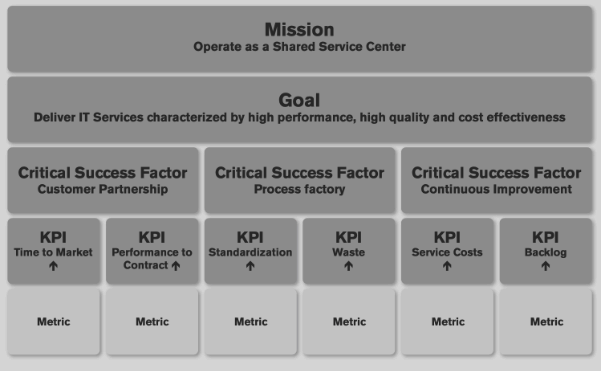
\includegraphics[width=0.8\textwidth]{images/vision.png}
    \caption{what to do}
    \label{fig:whattodo}
\end{figure}
